\documentclass{report}

\usepackage[a4paper, tmargin=2.54cm, bmargin=2.54cm, lmargin=3.17cm, rmargin=3.17cm]{geometry}
\newcommand{\head}[1]{\textnormal{\textbf{#1}}}

\usepackage{titlesec}    % Remove the text 'Chapter' from each chapter.
\titleformat{\chapter}{\normalfont\huge\bf}{\thechapter}{20pt}{\huge\bf}

\title{Bachelor's thesis \the\year}
\author{authors}
\setcounter{tocdepth}{3}
\renewcommand{\figurename}{Figure}
\renewcommand{\listfigurename}{List of Figures}
\usepackage{graphicx}
\usepackage{booktabs}
\usepackage{natbib}
\usepackage{xcolor}
\usepackage{helvet}

% %MORE PACKAGES HERE 

\begin{document}

%%%%%%%%%%%%%%%%%%%%%%%%%%%%
%%%% FIRST PAGE
% thesis' title, and supervisors

\begin{titlepage}
    \hspace{-1.5cm}
	
\includegraphics[width=50mm]{assets/logoAtrato.png}
	\hfill
	
\includegraphics[width=40mm]{assets/Hochschule-esslingen.svg.png}
	
	\noindent\begin{small} \sffamily
		\begin{minipage}{0.65\textwidth}
			Hochschule Esslingen University of Applied Sciences\\
			Atrato Technologies\\
			Winter Semester \the\year\\
			Degree thesis, 30 Credits\\
		\end{minipage}
	\hrule
	\end{small}

	%Thesis title
	\vspace{1cm}
	{\LARGE\noindent \textbf{Progressive automation of disbursement processes through integration with the Mexican digital banking system} \par}
	\vspace{0.5cm}
	%Thesis subtitle
	{\Large\noindent DHIK Double Degree: ITESM - Hochschule Esslingen | Faculty of Mechatronics and Electronics \par}
	\vspace{2cm}
	%Author's name
	{\LARGE\noindent Author: José Carlos Toscano Alcalá \par} %%%%% CHANGE STUDENT HERE

	\vfill
		
	\hrule
	\vspace{0.3cm}
	
%%% CHANGE SUPERVISORS AND REVIEWERS BELOW
	
	\begin{table}[h!]
		\begin{small} \sffamily
			\begin{tabular}{p{0.2\textwidth}p{0.8\textwidth}}
				Author: & José Carlos Toscano Alcalá \\
				Main Supervisor:    & Prof. Dr. Markus ENZWEILER, \\
				& Department of Computer Science and Engineering, Hochschule Esslingen \\
				Co-supervisor:      & Juan Pedro Casián Porter \\
				& Department of Product Development at Atrato, Atrato \\
				
			\end{tabular}
		\end{small}
	\end{table}
	
\end{titlepage}

\newpage
%%%%%%%%%%%%%%%%%%%%%%%%%%%%
% QUOTE
%%%%%%%%%%%%%%%%%%%%%%%%%%%%
\hspace{5cm}

\begin{quotation}
    “The first rule of any technology used in a business is that automation applied to an efficient operation will magnify the efficiency. The second is that automation applied to an inefficient operation will magnify the inefficiency.”
\end{quotation}
-Bill Gates


%%%%%%%%%%%%%%%%%%%%%%%%%%%%
% ABSTRACT
%%%%%%%%%%%%%%%%%%%%%%%%%%%%

\chapter*{Abstract}

With the growth in Atrato’s customers and partners consuming its main financial product, the number of loans granted on a daily basis has increased and the manual money disbursement process has become an exhaustive, repetitive, and error-prone task. 
In order to ensure a scalable and reliable disbursement procedure, this should progressively migrate to a fully automated activity compatible with current processes.
To track and monitor the complete disbursement procedure, a Balance System was built enabling an understanding of both a merchant's balance in a general and in a very granular way, implementing a logging system to ensure detailed visibility and traceability of the full process, integrated with existing Identity and Access Management modules for internal security.
 Connecting this Balance System to the entity provider of the access to the Mexican digital banking system through a custom API and web services for incoming updates and a private network. All this implementation considers certain flexibility on the disbursement modalities and was developed through Object Oriented Programing Principles, managing models and controllers, to ensure the best programming practices and a correct integration with the current Business rules, processes, and models.\\

 \textbf{Keywords: }\textit{Balance system, Buy Now Pay Later, disbursement, automation, compatibility}

%%%%%%%%%%%%%%%%%%%%%%%%%%%%
% PREAMBLE
%%%%%%%%%%%%%%%%%%%%%%%%%%%%

\chapter*{Preamble}

\subsection*{Foreword}
Lorem ipsum dolor sit amet, consectetuer adipiscing elit. Proin in diam. Nam dignissim facilisis lorem. Aliquam orci ipsum, egestas non, pretium at, venenatis in, felis. Pellentesque pellentesque. Vivamus in mi. Suspendisse cursus, augue quis malesuada mollis, massa lorem accumsan est, sed vulputate est nibh id pede.

\subsection*{Acknowledgements}
Lorem ipsum dolor sit amet, consectetuer adipiscing elit. Proin in diam. Nam dignissim facilisis lorem. Aliquam orci ipsum, egestas non, pretium at, venenatis in, felis. Pellentesque pellentesque. Vivamus in mi. Suspendisse cursus, augue quis malesuada mollis, massa lorem accumsan est, sed vulputate est nibh id pede.

\subsection*{Notations and conventions}
Explicar de UML, diagramas, mayusculas para objetos y entidades, cursivas para tipos



\tableofcontents

% %%%%%%%%%%%%%%%%%%%%%%%%%%%%
% % LIST OF ABBREVIATIONS
% %%%%%%%%%%%%%%%%%%%%%%%%%%%%

% \chapter*{List of Abbreviations}

% %%%% In alphabetical order
% BRB - Be Right Back\\
% IMHO - In My Honest Opinion\\
% L8r - Later\\
% LOL - Laugh Out Loud\\
% OMG - Oh My God!\\
% ROFL - Rolling on the Floor Laughing
% \addcontentsline{toc}{chapter}{List of Abbreviations}

% %%%%%%%%%%%%%%%%%%%%%%%%%%%%
% % LIST OF FIGURES
% %%%%%%%%%%%%%%%%%%%%%%%%%%%%
\listoffigures
\thispagestyle{plain}
\addcontentsline{toc}{chapter}{List of Figures}

% %%%%%%%%%%%%%%%%%%%%%%%%%%%%
% % LIST OF TABLES
% %%%%%%%%%%%%%%%%%%%%%%%%%%%%
% \listoftables
% \thispagestyle{plain}
% \addcontentsline{toc}{chapter}{List of Tables}
% % \addtocontents{toc}{\bigskip}

% %%%%%%%%%%%%%%%%%%%%%%%%%%%%
% %%%%%%%%%%%%%%%%%%%%%%%%%%%%
% % MAIN THESIS
% %%%%%%%%%%%%%%%%%%%%%%%%%%%%
% %%%%%%%%%%%%%%%%%%%%%%%%%%%%

|\chapter{Introduction}


\section{Motivation}

Throughout the development of Atrato’s main product, a Buy Now Pay Later (BNPL) financial service, many tasks and processes have been automated to enable a fast and efficient response to the final customers. Nonetheless, after-signature processes still were handled manually by an overcharged treasury team, handling more than 1,000 daily operations regarding money disbursements and credit cancelations. A process that became very time consuming, human-error prone and unsustainable at a larger scale. Atrato’s BNPL was very efficient to the end users but started to generate plenty of friction and operational load to the partners and operational side.\\

As Atrato’s market started expanding, new partnerships with bigger and more relevant merchants required efficient and flexible processes not only for the end user, but also for every new merchant that joins Atrato as a partner. Atrato’s partnership with what today is their biggest merchant demanded immediate disbursements after every approved purchase. Not only immediate bank transfers needed to be handled, but also the process of managing credit updates and cancelations needed to be very efficient. To enable this partnership to happen, a balance system needed to be developed, capable of managing bank transfers with flexible triggers and handling changes in previous credits or cancelations.


\section{Starting points}

Before the development of the balance system for merchants and stores, Atrato was able to receive payments through different providers and manage the money properly.  In terms of taking money out of Atrato’s banking account and sending it to a different account only the treasury team, composed by 2 people, was able to do this task. After confirming that the money was disbursed correctly, they proceeded to update every credit, adding a flag that indicates that the credit was already disbursed. After this, a manual spread sheet was generated to send it as a disbursement report to every merchant and store.\\

Regarding each merchant’s banking information, none of it was saved as part of the information stores while adding a new merchant. All of it was later requested by the treasury team, making that the information needed for an automatic disbursement was not centralized. Additionally, every bank account needed to be authenticated before transferring a credit’s disbursement for security purposes.\\

In terms of how much money needed to be transferred per credit, it could always vary depending on every merchant’s current commission or if any special promotion or discount is active as part of the commercial team. All these factors needed to be considered before making a money disbursement. Furthermore, every new merchant could go through a trial period, where very specific commissions apply and would later change depending on its monthly origination. \\

This poorly structured process was the starting point before any automation could be developed, where current business processes should be able to continue operating in a similar way as they were already doing.\\

Concerning technical starting points, Atrato’s codebase has been slowly migrating from functional programing, developed in JavaScript, to an Object-Oriented Programing structure in Typescript. All data is stored and handled in a single relational database with MySQL as the engine but consumed through TypeORM, an Object-relational mapping (ORM), allowing a Model-Controller-Router Structure for the server side.\\


\chapter{General overview}


\section{Current business pipelines}

It is very important to understand existing processes before attempting to automate these tasks. Atrato has partnered up with numerous merchants with possibly more than one store throughout Mexico. Every single partnership was discussed and agreed upon different terms, resulting in different expectations regarding how the money will be disbursed once a credit is granted through Atrato’s application process. These processes could either be monthly, weekly, daily, or individually per credit. Additionally, merchants could be conditioned to specific commissions depending on different factors like their monthly origination or if they were on a specific trial period. All these rules were not specifically written down nor followed any guideline. This meant that every time a disbursement needed to be made, the person in charge should review every commission agreed and compute the merchant’s monthly origination to know exactly what amount and in what conditions should the disbursement be made.

\subsection{Understanding Atrato’s Partners, Merchants and Stores}

Atrato’s partners are those commercial allies that offer its Buy Now Pay Later service as part of their payment options. These partners are internally classified as Merchants and each of these merchants could have 1 or more registered Stores.\\

The application process for a loan with Atrato takes place through Atrato’s web application by filling in information about the customer’s personal profile and financial information, indicating the Merchant and Store in which the loan will take place. Once the application is fully authorized by Atrato and the customer has finished the signature of its digital contract, then the store proceeds to deliver the product to the customer. Now, depending on the type of disbursement agreed upon the merchant’s registration the money regarding the purchase will be transferred to the merchants banking account. This describes the process for a single application, but multiple applications need to be handled both by Atrato’s partners and Atrato’s internal team.

\subsection{Disbursement process}
The disbursement of a credit could be as simple as taking the amount of the credit and transfer it to the bank account related to the merchant. The complexity is added when a merchant does not want to receive plenty of bank transfers per day or even per week and rather have all the money disbursed as a single transaction at the end of the month. Since every partner expects this task to be handled upon their own agreed terms every bank transfer needs to be carefully reviewed. Additionally, just like a partner can have their own terms, Atrato has its own specifications and requirements to every partner. Some commissions may be included to the partner depending on their specific monthly origination and type of partnership. Furthermore, already disbursed credits could be later canceled or a change in amount may happen for many reasons, leading to a negative balance with merchants.\\

Taking all these factors into account, a money disbursement is made firstly depending on the expected disbursement periodicity, then the total amount to be transferred is computed depending on the number of credits and their commission and this amount is manually sent in a single bank transfer.\\

Once the bank transfer is successfully confirmed a report is generated indicating every credit that was part of the disbursement, their corresponding commission and any change in amount or cancelation that was taken into account to compute the total amount. This report is then sent to every single merchant enabling complete transparency and understanding of every bank transfer that is sent.
\subsubsection{Partner’s dashboard}
Every partner has access to an internal dashboard where they can visualize and manage their customers’ applications and give follow ups on each product’s delivery or cancelation. The money regarding a new credit will not be disbursed until the partner notifies the delivery of the product through their dashboard. This notification works as Atrato’s triggering event to dispatch the money disbursement, the process that is intended to eventually be fully automated. This process is very important to be sure that no credit is disbursed before they are marked as “delivered”. Once the credit’s product is delivered the partner can visualize when the credit is disbursed. This dashboard is helpful to compare the information received from the disbursement’s report and what they visualize as the credits that were already delivered and disbursed.

\subsection{Compatibility with current business and application processes}
An active customer’s application turns into a credit once the information is validated every required document is uploaded and an offer is sent. If the customer agrees to the term’s presented in the offer, then it goes through a digital signature process, where all the details of the credit can be confirmed. Once the signature is generated the credit is finally created. It is in this moment where the calculations for the credit’s commission need to be made to know exactly on what terms was this credit granted. The existing architecture supported a static commission per merchant, which was immediately assigned to the credit, but not necessarily represented the correct commission.\\

A merchant’s commission could change every month depending on the previous month’s origination. Furthermore, depending on the type of merchant the commissions could vary even depending on the number of payments agreed for the credit. Temporary promotions should also be considered in the process before deciding the exact commission for every credit, where a specific deal for interest free months for the end customer could represent a higher commission for the merchant offering this promotion.\\

All these factors must be considered before attempting to automate the disbursement process, without implying a change on current application or business processes.\\

Every agreed commission, trial period and origination thresholds for every merchant should be saved in a standardized manner, enabling a better understanding and implementation of the agreed terms.

\section{Automation of disbursement process requirements}
The first step towards this automation should creating a detailed pipeline of the process. Every task and validation that was manually done before transferring a partner’s origination to their bank account will now need to be defined and structured in a regulated process.\\

The automation of such a delicate process can be achieved through the development of a modular Balance system for each of Atrato’s partners. This balance system should be completely traceable. This means that we should be able to know what is happening all the time, exactly how the computations are made and every factor that is affecting a partner’s balance. It should be able to be handled independently for each partner with the possibility to disable the automation for some of them at any moment. A security step should be implemented, where some balance systems could require a manual confirmation of the bank transfer before it is sent. This could be helpful for transitioning from a manual process with some partners into the whole automation pipeline. \\

Additionally, an integration with Banco de Mexico, the Mexican Banking System regulatory agency is needed to handle bank transfers properly. Since Atrato has not yet the technology to independently make bank transfers from one account to another this integration will be done through a third party that provides all access and security that is required.

\section{Balance system for partners}
This system should be modular enough to handle even different Bank Accounts per merchant. Since every merchant could have different stores, the modularity of the banking system will be done individually per every store.\\

The system will describe every update to the store’s balance, enabling a complete understanding of how any contribution to the balance was made or how it was adjusted. It will relate every credit generation or cancelation, every money disbursement, and every manual adjustment to the ongoing bank transfers.\\

The balance system will be handled through Balance Update object which will eventually generate Bank Transfer objects all of which will be triggered by some specific requirements. In the following sections we will get a general overview of these models. 

\subsection{Balance Updates}
A Balance Update will be every movement, transaction, adjustment, or cancelation that directly affects the system’s balance. Balance Updates serve as the linking entity between a confirmed credit and a store’s balance considering the appropriate commission. Every Balance Update will contribute in a way to the general balance, recording the previous balance and the new balance after its contribution. In this way, to effectively know the system’s current balance it would be enough to inquire the last Balance Update.\\

Balance updates can be created through the confirmation or cancellation of a new credit, through the confirmation of a successfully disbursed Bank Transfer or through the cancelation of a previously confirmed disbursement. Furthermore, a Balance Update could be generated manually by the treasury team whenever a Balance Adjustment is required. Furthermore, Balance Updates could have different specifications, expected behaviors or status updates depending on their type. These specifications will be furtherly discussed in Chapter 3.

\subsection{Bank Transfers} 
A Bank Transfer object will be the entity describing the money movements between Atrato’s bank account and every store’s bank account. Bank Transfers will only be generated through and composed by Balance Updates and their status will be directly related. Once one or more Balance Updates are linked to one Bank Transfer, they will not be able to be related to any other Bank Transfer. Once the Bank Transfer is sent through the online banking system and the confirmation is received a new Balance Update will be generated indicating the money disbursement, or the corresponding updates in the Balance Updates’ status will be handled according to any possible cancellation.

\subsection{Triggers}
Atrato’s partners require specific disbursement processes, whether it is a daily, weekly, or monthly disbursement of the credits approved during this period or an immediate disbursement per credit. To allow this flexibility, the generation of a Bank Transfer will be initiated through specific triggers. Every store can have one of the following disbursement types: Instant, Hourly, Weekly or Daily.\\

These four disbursement types will be triggered accordingly through Cron Jobs. Once these events are triggered, all pending Balance Updates will be considered for generating a new Bank Transfer only if the total amount of these pending Balance Updates is higher than the minimum amount required for a Bank Transfer. This threshold is defined to avoid sending Bank Transfers with a low amount of money, since every banking transaction also represents a cost for the company. There may be some edge cases where the total amount of the pending Balance Updates is even lower than \$0.00, this just means that for some reason the system’s balance is negative and no money will be disbursed until the balance becomes positive again through the origination of more approved credits or any further update to the store’s balance. Note that all these updates can only be done through Balance Update object.

\subsection{Understanding the correct handling of partner’s commissions}

Every merchant, as well as every store, has a standard commission. All the business logic regarding the correct amount for these commissions should be handled independently to the automatic disbursement process. \\

Commissions can change dynamically depending on different factors, like special promotions, discounts or regarding the merchant’s monthly origination. All these process and specifications should not interfere with the automatic disbursements. Every credit must have a commission assigned before it can be approved for disbursement. This will be the commission that will be considered for the computation of the amount for the Balance Update generated by the approval of a credit. \\

Independently of how a partner’s commissions vary, since the commission is directly assigned to the credit, these two business processes will not interfere with one another.

\section{Refactor and Changes}

Current business processes and the existing models for merchants, stores and all the structure for selecting a credit’s loan term where not able to support a new system where disbursements could be automated. Since the disbursement of a credit is the missing link that could complete the full automation of the credit application and lending process, all the entities involved converge in this point and some of them will require some very specific changes: A store’s bank account should be validated and ready to receive payments, a credit’s commission should be able to be determined according to the term selected, the amount requested and any applicable promotion that could be involved. Hence, additional to the changes in current pipelines that are required, a complete re-design of the architecture related to how a customer could select the conditions of the loan they are applying to must be done.

\subsection{Registration of merchant’s pipeline changes}

During the registration process of any new merchant and their corresponding stores involved, the banking information of the stores should now be a required field. Once a merchant is added, its first store should be added as well, and every time a store is added its banking information should be included.\\

The Treasury team oversees validating a merchant’s commission depending on the terms agreed upon their registration. To do this, a new attribute, isValidated, will be added to both the Merchant and the Store models indicating if the information has already been validated by the Treasury team. This extra validation step is now included as part of the registration process of a merchant. Every time the information of a merchant or a store is added or edited, the isValidated flag will be set back to false, indicating that a new validation of the Treasury team is needed.\\

The whole registration pipeline is mounted in a dashboard developed for internal use with CRUD operations. With any subtle change in the Update method, as shown in the code snippet below the isValidated flag will always turn back to false when used, requiring an additional validation.

\begin{verbatim}
    await getRepository(Merchant).update(
        merchantId,
        {
         ...merchant,
         isValidated: false,
        }
       );
       
\end{verbatim}

A merchant cannot be validated if it does not have at least a validated store. Furthermore, any merchant that is not validated will not be displayed as an option in the application form.  Additionally, a new Model will be introduced: Payment Option. Its connection to the Merchant-Store model will be described in the following section.

\subsection{Refactor in partiality selection architecture}

During the development of Atrato’s customers’ application process the commissions for the merchants where not considered. Furthermore, with the iteration of commercial and partner acquisition processes a credit’s commission became more complex. A credit’s commission can depend on the number of payments, the credit’s amount, and ongoing promotions. To enable this dynamism a refactor of the internal architecture of the term selection options needed to be done.\\

Previously, whenever a merchant was incorporated to Atrato’s partners a simple setup of the available terms was done. At this moment we only kept a record of the possible number of payments that were available for this merchant’s stores. Be it a range from 3 to 24 monthly payments. We needed to elaborate every merchant’s term options into a whole module of Payment Options, where every payment option includes specific interest rates depending on a customer’s risk profile, the number of payments, the requested amount and had expiring dates in order to work as promotions. In this way the Payment Options module could support flexibility and the availability of every option could be determined through a customer’s input.\\

This Payment Option model will refer to all the possible terms that a store could have and will include details regarding specific interest rates that could vary depending on a customer’s risk profile, and will include applicability filters for date and requested amount, the option to be tagged as a promotion, specifications on the specific merchant’s commission, a trial period specification and very importantly a flag indicating if its commission could be automatically updated to integrate with the on-going changes in a merchant’s commission due to their monthly origination. Please refer to 2.4.2.2 Payments Options UML for specific details on the model.\\

Payment Options will also go through the validation step from the Treasury team, following the same structure and process as before. Every store should have at least a validated Payment Option before being completely validated. Now, the complete pipeline goes as follows:\\

Whenever a merchant is added, its first store should also be added, and the first payment option for the store should be added as well. Regarding the validation process, it goes the other way around, payment options should first be validated before attempting to validate a store, and once a store is validated the merchant can be validated as well. All of these is just as a general validation to make sure that there is no merchant that does not have a valid store and that every valid store has at least a valid payment option.

\subsubsection{Diferences between Payments Per Store and Payment Options architecture}

\begin{figure} [h]
    \centering
    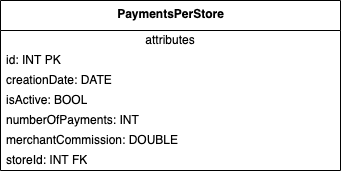
\includegraphics[scale = 0.6]{assets/uml/Payments_Per_Store.png}
    \caption{Payments Per Sotre UML}\label{fig:uml_payments_per_store}
\end{figure}

With the Payments Per Store Model a commission could directly be mapped to a specific number of payments, but there exists zero flexibility regarding a change of commission depending on the requested amount nor any distinction between a regular term or any offered promotion. Furthermore, interest rates need to be handled independently and could not directly be related to the number of payments that a customer selects.

\begin{figure} [h]
    \centering
    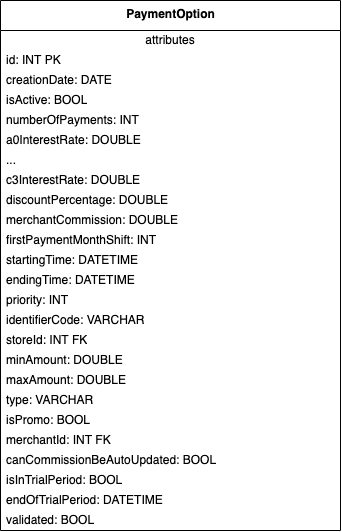
\includegraphics[scale = 0.6]{assets/uml/PaymentOptions.png}
    \caption{Payment Option UML}\label{fig:uml_payment_options}
\end{figure}

Pending: 	
Add details and describe how payment options work and how they enable the flexibility that was needed regarding the commissions and interest rates….


\chapter{Development of the Automated Balance System}

\section{Development of module through OOP, managing models and controllers}

As discused before, the core elements composing a store's balance system are Balance Updates and Bank Transfers. These elements are constructed as Models, which in terms of OOP are represented by Classes. These Classes' attributes and elements will be handled independently by Models and Controllers Classes. Every action or method regarding the models will be handled by the Controllers.\\

The Controllers will generate instances of the Balance Updates and Bank Transfers models and handle the relationships between them. They will serve as the link between the application and the Database as well by using TypeORM Repositories for these Models.

These controllers classes handle different actions and processes within them and where designed toin such way that their methods always return a specific interface as their response. This interface is called \textbf{\textit{ControllerResponse}} and it will either be a successful or unsuccessful response. This will be identified with the attribute \textit{success}. For successful responses, the attribute \textit{res} will be included and its type will be described by the generic indicator \textbf{\textit{T}}. In the other hand, for any unsuccessful response, the attribute \textit{error} will be included containg an object in the form of a \textbf{\textit{ControllerError}} as follows:

    
    \begin{verbatim}
        
        type ControllerResponse<T> =
        | {
            success: true; 
            res: T;
            }
        | {
            success: false;
            error: ControllerError;
            };
            \end{verbatim}
            
A \textbf{\textit{ControllerError}} will contain additional details as a string describing the specific expection making it compatible with Javascript's Error type:
            
    \begin{verbatim}
        interface ControllerError {
            msg: string;
            }
    \end{verbatim}
                

    \subsection{Balance Updates}

The System's general balance will be composed by numerous Balance Updates. Where the changes in the balance of the store will be reflected on each of them. As shown in Figure \ref{fig:uml_balance_update}, every instance will have its own \textit{id} as primary key, which will serve as reference for any foreign key relationship. The atribute \textit{amount} indicates exactly how the store's balance will be updated, keeping a record of the store's previous balance and the current balance after the update was added in the respective attributes.

\begin{figure} [H]
    \centering
    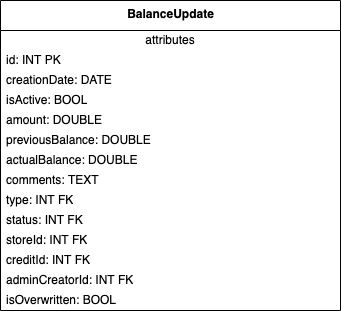
\includegraphics[scale = 0.7]{assets/uml/BalanceUpdate.png}
    \caption{Balance Update UML}\label{fig:uml_balance_update}
\end{figure}

Every Balance Update must have a \textit{storeId} foreign key, indicating which store's balance it is affecting.\\ 

The attribute \textit{creditId} will serve as a reference for linking a credit entity to the Balance Update it created when it served as a \textit{Contribution} or \textit{Credit cancelation} to the store's balance. These refere to the types that a Balance Update could have and will be furtherly explained in the following section.\\

Some Balance Updates could be manually generated by any administrator with the appropiate permissions. For this scenario, it is important to keep a record of who made these changes by saving this administrator's id in the attribute \textit{adminCreatorId} and label these changes with the respective \textit{type}. 


\subsubsection{Balance Updates Types}

Every Balance Update will have a specific \textit{type} attribute. These types are managed as a table with static values and referenced through their \textit{id} attribute. Every Balance Update presents the same behaviour independently from their \textit{type}, nontetheless, they represent specific changes and reasons for these changes that do depend on the \textit{type} they have. For this reason, the type can not be edited once the instance of the Balance Update is generated. The different possible types of Balance Updates are described in Figure \ref{fig:balance_updates_types} 

\begin{figure}[H]
    \caption{Balance Update Types}\label{fig:balance_updates_types}
    \begin{tabularx}{1\textwidth} { 
    | >{\centering\arraybackslash}X 
    | >{\centering\arraybackslash}X 
    | >{\raggedright\arraybackslash}X | }
   \hline
   id & Type & Description \\
   \hline
   1 & \textit{Contribution} & Contribution to balance due to a new credit   \\
   \hline
   2 & \textit{Disbursement} & Disbursement generated through the confirmation of a Bank Transfer   \\
   \hline
   3 & \textit{Credit Cancelation} & Loads negative balance due to credit cancelation   \\
   \hline
   4 & \textit{Adjustment} & Loads adjustment in balance to be considered in the next Bank Transfer   \\
   \hline
   5 & \textit{Disbursement override} & Overrides the amount addedd to the balance from another Disbursement   \\
  \hline
\end{tabularx}
\end{figure}

\subsubsection{Overwriting Balance Updates}


Balance Updates have an attribute to indicate if the object was overwritten. Whenever an object is overwritten, this means that there is an additional Balance Update that is cancelling its affectation on the store’s general balance. This is particularly helpful to keep control of a store’s balance modification for those scenarios where there are involved some cancelations, overrides or any manual adjustment. The only Balance Updates that could be overwritten are those of the types of \textit{Disbursement} and \textit{Contribution}.\\

A Balance Update of type \textit{Disbursement} is generated whenever a confirmation that a Bank Transfer has been successfully accepted is received. There are some edge cases where this \textit{Disbursement} Balance Update needs to be overwritten for external reasons; this could happen, for example, due to the cancelation of a Bank Transfer. Furthermore, there is a very rare, but possible, scenario where the money could be returned even after it was confirmed, but the expected outcome is just as that of a cancellation. For these cases, the Disbursement that was generated is no longer valid, hence, an update to the store’s balance should be made. This is done by generating an additional Balance Update with type \textit{Disbursement Override} as shown in Figure \ref{fig:override_disbursement}. This new Balance Update will contribute once again the amount that was previously reduced to the store’s balance.\\

\begin{figure} [H]
    \centering
    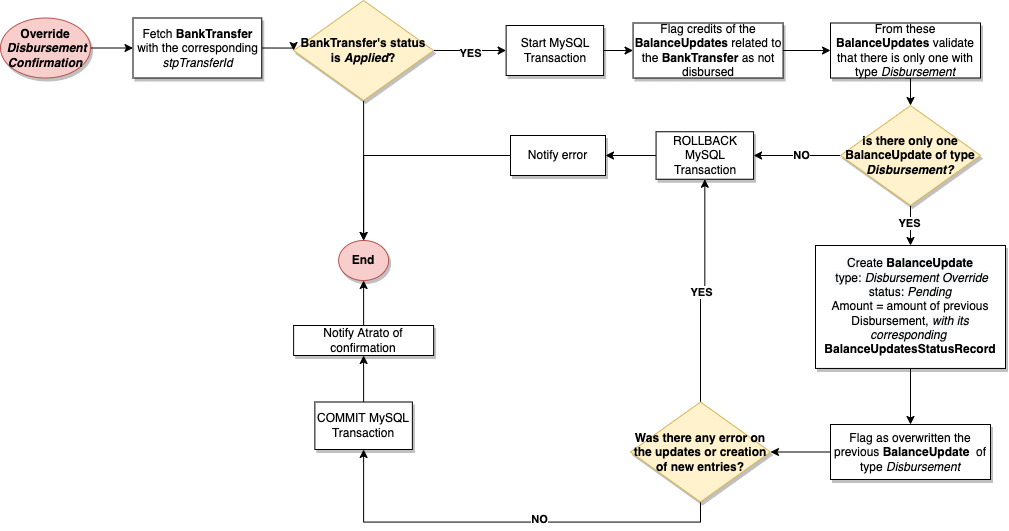
\includegraphics[scale = 0.4]{assets/diagrams/DisbursementOverride.png}
    \caption{Process for overriding a previously confirmed Balance Update of type Disbursement}\label{fig:override_disbursement}
\end{figure}


Furthermore, Balance Updates of type Contribution could also be overwritten at some point. These are created once a partner has confirmed a product’s delivery through their dashboard and the credit of that product will generate a contribution to the store’s balance. This means that there is some amount that Atrato must eventually transfer to the partner’s bank account depending on the disbursement modality that this partner has active. These contributions could eventually be overwritten if the credit is later cancelled. For this particular scenario, a new Balance Update of type \textit{Credit cancelation} needs to be created to compensate the previous contribution, regardless of the contribution’s status as shown in Figure \ref{fig:dlowchart_credit_cancelation}.


\begin{figure} [H]
    \centering
    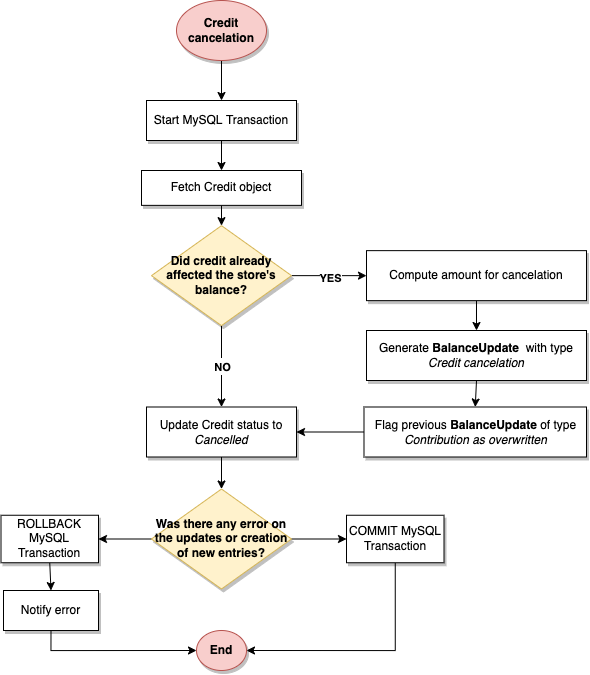
\includegraphics[scale = 0.6]{assets/flowcharts/CreditCancelation.png}
    \caption{Processing a credit's cancelation and its affectation to a store's balance system}\label{fig:dlowchart_credit_cancelation}
\end{figure}

\section{Bank Transfers}

Just as the Balance Updates, as shown in Figure \ref{fig:uml_bank_transfers}, every Bank Transfer will have their primary key \textit{id}, useful for any foreign key relationship, and a not nullable \textit{storeId}. The attribute \textit{status} will internally describe wether the Bank Transfer has already been sent, confirmed, cancelled or rejected, while the attribute \textit{stpStatus} will be the value received upon any incoming update regarding the payment order related to this Bank Transfer. The status of the Bank Transfers can not be arbitrarily updated from one status to another one, the specific expected behavoiour will be furtherly discissed in Chapter 4.
The \textit{dispersionDate} will indiacte the date when the Bank Transfer was dispatched as a payment order. This dispatch could be either done automatically or through a manual confirmation, hence, it will no necesarily be the same as the \textit{creationDate}. Furthermore, the \textit{trackingKey} will be the attribute used to link the Bank Transfers objects and the payment orders from STP.

\begin{figure} [H]
    \centering
    
\includegraphics[scale = 0.7]{assets/uml/BankTransfers.png}
    \caption{Bank Transfer UML}\label{fig:uml_bank_transfers}
\end{figure}

\subsection{Generating Bank Transfer objects}

Once the trigger for generating a new Bank Transfer is received, the store's current balance will be used as the Bank Trasfer's amount. As shown in Figure \ref{fig:bank_Transfer_trigger}, all the Balance Updates with status \textit{Pending} will be related to the new Bank Transfer and will then update their status to \textit{In transit}. An additional confirmation could be added at this point for those stores where the Bank Transfers must be confirmed manually by the Treasury team. If this confirmation is not necessary, then a new paymenr order can be generated and sent through STP using the information of the Bank Transfer. This process will be furtherly described in Chapter 4. Once the Bank Transfer has been succesfully sent as a payment order, then a new Balance Update of type \textit{Disbursement} will be generated to appropiately update the store's balance and the credits related to any of the Balance Updates from this Bank Transfer can now be flagged as \textit{disbursed}.\\

\begin{figure} [H]
    \centering
    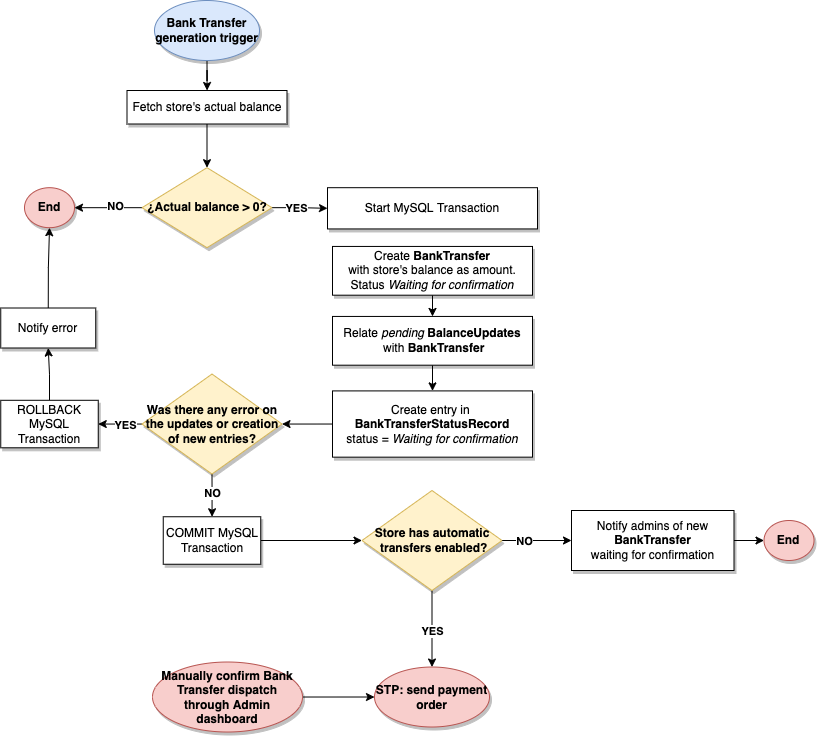
\includegraphics[scale = 0.4]{assets/flowcharts/BankTransferTrigger.png}
    \caption{Bank Transfers generating trigger}\label{fig:bank_Transfer_trigger}
\end{figure}

The process of actually sending the payment order through STP will be furtherly described in Chapter 4.\\

\subsubsection{Status updates records}

Every time that the internal status of a Balance Update or a Bank Transfer is updated a record will be generated to keep track of every update. As shown in previously shown diagrams, these records will be stored in the entities Bank Transfer Status Update Record and Balance Update Status Record respectively. Even though the status entities are equal in sturcture, they will be handled independently, for this reason the status updates records are handled independently as well.
These status records will simply keep track of the next status of any Balance Udpdate or Bank Transfer, as shown in Figure \ref{fig:status_record_uml} the creation date of the record will indicate the moment where the status was updated. For new instances of Balance Updates or Bank Transfers, a status record will be created with the initial status. 

\begin{figure} [H]
    \centering
    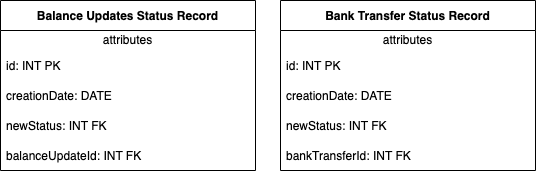
\includegraphics[scale = 0.6]{assets/uml/StatusRecordUML.png}
    \caption{Status Record UML for both Balance Updates and Bank Transfers}\label{fig:status_record_uml}
\end{figure}

Since a Bank Transfer is composed of multiple Balance Updates, then their status updates are directly related. Figure \ref{fig:bu_state_machine} describes how the status of any Balance Update could change depending on how the Bank Transfer's status changes. 

\begin{figure} [H]
    \centering
    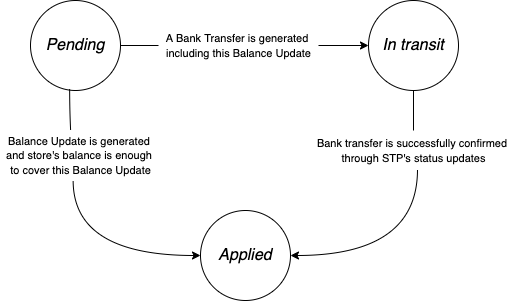
\includegraphics[scale = 0.6]{assets/diagrams/BUStateMachine.png}
    \caption{Balance Updates State Machine related to changes in their related Bank Transfers}\label{fig:bu_state_machine}
\end{figure}

Note how once a Balance Update is updated to the status \textit{Applied}, then it can not be updated furtherly; this is a final status. Any additional update regarding any confirmed Balance Update should be represented as a \textit{Cancelation}, Disbursement \textit{Cancelation} or \textit{Manual adjustment}, but the Balance Updated that was already applied will not produce any additional change in the store's balance.


\section{Ensure correct functionality and error handling through MySQL Transactions}

As noted in the diagrams exposed in previous sections, a particullar service from MySQL, called Transactions, is implemented for updating and inserting new entities to the databes. This database service, powered by Oracle, refers to a safe update functionality. These transactions enable running a group of statements, commonly used for inserting or updating data, with the possibility to discard all changes if required. This behaviour could be particularly usefeul when performing a large amount of updates or inserts within a large process. If any command fails for whatever reason, then all the previous updates should be rollbacked, resulting in a complete failed process instead of a partial failed process. Either every update is executed as expected or none of them are. The general structure of a MySQL Transaction is displayed in the following code snippet available from Oracle's official MySQL Reference Manual \cite{mysqldocs}

\begin{center}
    \begin{verbatim}
        START TRANSACTION;
        SELECT @A:=SUM(salary) FROM table1 WHERE type=1;
        UPDATE table2 SET summary=@A WHERE type=1;
        COMMIT;
    \end{verbatim}
\end{center}

Every transaction must start with the command \textit{START TRANSACTION}. Every following statement will run within the scope of the Transaction. Changes to the tables in the databse will not be made permanent immediately, since they must either commited or rollbacked. The \textit{COMMIT} statment will save the changes to disk while the \textit{ROLLBACK} command will ignore them. \cite{mysqldocs}\\

To enhance this funcionality and to make it compatible to the ORM Atrato is handling, a single connection must be assured will executing any transaction. TypeORM supports Transactions through the implementation of QueryRunners, specifically to create and control state of single database connection. A single QueryRunner instance must be created to handle a single Transaction.\cite{typeorm}\\ 

To instantiate a QueryRunner from TypeORM first the connection should be fetched. Once the QueryRunner is created and successfully created the single database connection, then the Transaction can be started. This process can be executed as follows:

\begin{verbatim}
    const connection = getConnection();
    const queryRunner = connection.createQueryRunner();
    await queryRunner.connect();
    await queryRunner.startTransaction();
\end{verbatim}

Once the transaction has been started within the scope of the QueryRunner, the correct Commit or Rollback should be handled appropiately. Once the transaction has been succesfully terminated, the Query Runner can be released.\cite{typeorm}

\begin{verbatim}
    // Only one of the following methods should be executed before releasing
    // the query runner
    await queryRunner.rollbackTransaction();
    await queryRunner.commitTransaction();
    // Release the single connection
    await queryRunner.release();
\end{verbatim}

The entire Balance System is composed by different events and triggers that could initiate specific processes where not only BalanceUpdates and BankTransfers, but also some Credit instances must be edited or added to the database. A correct functionality must be ensured and none of these processes should be partially completed. In other words, the creation and dispatch of a Bank Transfer must be donde successfully, with the corresponding state updates and records of these state changes. If an error occurs during any process, then the entities involved should not be edited, nor any additional entity should be created. The error could be later reviewed and the process could be repeated once again, replaced or even discarded. This expected behaviour also applies for handling the creation and update of the BalanceUpdates.\\

QueryRunners will be the base element managing all the updates and inserts within the complete Balance System. To apply correct design patterns and avoid repetition, a base controller class was developed to ensure that every method within the \textit{BankTransfersController} and the \textit{BalanceUpdatesController} could handle QueryRunners appropiately.

To ensure compatibility with Atrato's codebase and the Controllers' expected response, two methods where added in this base controller as described here: 

\subsubsection{Returning a successful Controller Response, handling the Commit and Release of the Query Runner's Transaction}

The method will take as a parameter the expected response to be returned and the Query Runner containing the single database connection. This method will simply assure that the existing Transaction will be commited and released before returning any successful response.

\begin{verbatim}
async returnSuccessWithCommit<T>(
       controllerSuccessfulResponse: T,
       queryRunner: QueryRunner
   ): Promise<{ success: true; res: T }> {
       await queryRunner.commitTransaction();
       await queryRunner.release();
       return { success: true, res: controllerSuccessfulResponse };
   }
\end{verbatim}

\subsubsection{Returning an unsuccessful Controller Response, handling the Rollback and Release of the Query Runner's Transaction}


Just like the successful response, the method will take as a parameter the Query Runner, but instead of having the expected response it will take as another argument the \textbf{\textit{controllerError}} created in any exception.

\begin{verbatim}
async returnErrorWithRollback(
       controllerError: ControllerError,
       queryRunner: QueryRunner
   ): Promise<{ success: false; error: ControllerError }> {
       await queryRunner.rollbackTransaction();
       await queryRunner.release();
       return { success: false, res: controllerError };
   }
\end{verbatim}

The combination of these methods compose the expected \textbf{\textit{ControllerResponse}} return interface for any Controller, as described at the begining of Chapter 3.

\section{Detailed visibility and traceability of full process}

The process being automated consists of very delicate matters, therefore, there should exist complete traceability of every action that was executed within the whole system. Every error presented during eny process should be able to be traced and identify easily in order ot take actions, as well as any process that was completed successfully. With this objective in mind, the Balance System was connected to an existing internal logging system, where every process interuption or completion is logged in the database with the respective data and payload necesary for identification.\\

Since all actinos regarding the database are hadndled through a QueryRunner, then this logging implementation should also considered these matters. Whenever process is completed and the changes will be commited, the log of this event should be included in the Commit. This applies equally for any action being rollbacked; the changes should e ignored by the trasnaction, but the log of the process should indeed be saved.

The logging system was integrated within the same Base Controller developed for handling Query Runners's transactions as follows:

For successful responses, the Log could be simply added as part of the existing transaction before commiting and releasing the connection as shown with pseudocode, refering to the implementation of the Successful and unsuccessful responses.

\begin{verbatim}
    async returnSuccessWithCommit<T>(
           controllerSuccessfulResponse: T,
           queryRunner: QueryRunner,
           processLog: Log
       ): Promise<{ success: true; res: T }> {
           // Save processLog to database
           await queryRunner.commitTransaction();
           await queryRunner.release();
           return { success: true, res: controllerSuccessfulResponse };
       }
\end{verbatim}

In the other hand, for unsuccessful responses the rollback should be done before adding anything extra to the trasnaction.  Once the trasnaction is rollbacked, the connection is still active, hence, normal statments can be executed which will be immediately applied.

\begin{verbatim}
    async returnErrorWithRollback(
           controllerError: ControllerError,
           queryRunner: QueryRunner.
           processLog: Log
       ): Promise<{ success: false; error: ControllerError }> {
           await queryRunner.rollbackTransaction();
           // Save processLog to database
           await queryRunner.release();
           return { success: false, res: controllerError };
       }
    \end{verbatim}

\section{Balance System Integration}

There are different events happening in Atrato's pipeline and business processes that could trigger some specific actions regarding the store's balance. The sytem could be affected either by updating the store's balance by adding new Balance Updates, or by generating bank Transfers objects from the existing Balance Updates. Furthermore, the status of these Bank Transfers could be updated, indicating some specific actions on the system. The existing events and triggers are shown in Figure \ref{fig:balance_system_triggers}.

\begin{figure}[H]
    \caption{Balance System Triggers}\label{fig:balance_system_triggers}
    \begin{tabularx}{1\textwidth} { 
    | >{\centering\arraybackslash}X 
    | >{\centering\arraybackslash}X 
    | >{\raggedright\arraybackslash}X | }
   \hline
   Event & Trigger & Description \\
   \hline
   \textit{Bank Transfer generation trigger} & Through Cron Job monitoring every store's disbursement type & Generates new Bank Transfer object with current's store balance [PENDIENTE]   \\
   \hline
   \textit{Contribution of new credit} & Notification of the delivery of a credit's product & Generates a Balance Update indicating the contribution to the stoere's balance  \\
   \hline
   \textit{Cancelation of credit} & Notification of the cancelation of a credit & Generates a Balance Update indicating the cancelation of the credit amount to the stoere's balance  \\
   \hline
   STP status update: \textit{Liquidated} & Through incoming activity in STP's webhook & Starts the confirmation process of a Bank Transfer   \\
   \hline
   STP status update: \textit{Cancelled} & Through incoming activity in STP's webhook & Starts the cancelation process of a Bank Transfer   \\
   \hline
   STP status update: \textit{Returned} & Through incoming activity in STP's webhook & Starts the rejection process of a Bank Transfer   \\
   \hline
\end{tabularx}
\end{figure}

    
Since most of these triggers happen as a result of automated processes or through actions from third parties, like merchants or STP's servive, to ensure the correct functionality of the balance system, Atrato must have a way of replicating these actions in case something external is not working as expected. Internally, any process executed as part of a web service or exposed endpoint to these third parties can also be executed by any administrator from Atrato with the required permissions.\\
    
The general integration of these events and triggers is described in Figure \ref{fig:balance_system_triggers}, displaying how the Balance Updates and the Bank Transfers in a Store's Balance System can be generated through distinct actions and how they relate between each other. Note how the only output of the system are the Bank Transfers generated as payment orders for the intrgration with STP's services Furthermore, STP will send updates on these payment ordrers' status and the system will then generate actions accordingly. Specifications on the integration with STP will be furtherly discussed in the following chapter.

\begin{figure} [H]
    \centering
    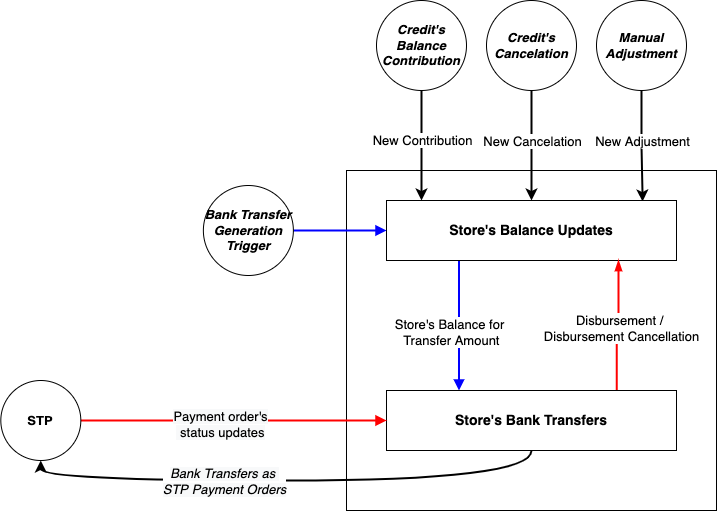
\includegraphics[scale = 0.5]{assets/diagrams/BalanceSystemDiagram.drawio.png}
    \caption{General integration of a Store's Balance System's triggers and internal processes}\label{fig:balance_systen_diaran}
\end{figure}

\section{Integration with current business processes}

Since the balance system is part of the general customer pipeline it must be directly integreated with current business processes. Once an application from a customer becomes an active credit, this credit could become part of the automated balance system of a store, depending if this store in particular has the automatic disbursements balance system enabled.\\

Furthermore, an existing credit could be affected through additinoal processes, like a change in the amount, a cancelation of the purchase or even a change of Store. The latter must be particularly addressed, since a credit could change from a store with its automatic system enabled to another one without it, or the other way around. The automation of any store's balance is completely integrated into every process to consider if the store has the system enabled or not before realizing any changes or updates to it. This behaviour is described in a general manner in Figure \ref{fig:automation_validation}, where this validation is included throughout every method of the Balance Updates and Bank Transfers Controllers.

\begin{figure} [H]
    \centering
    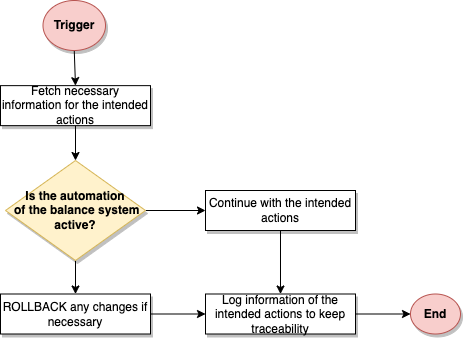
\includegraphics[scale = 0.5]{assets/flowcharts/AutomationValidation.png}
    \caption{General validation of Balance Updates and Bank Transfers Controllers' methods}\label{fig:automation_validation}
\end{figure}

\chapter{Access to the Digital Mexican Banking System}

\section{General Overview}

The Bank of Mexico regulates every transaction between different banking accounts in Mexico. To be able to gain access to their digital banking system Atrato partnered with another Mexican fintech, STP. STP stands for Payments and Transfers System in spanish, and they are part of the System of Interbank Electronic Payments (SPEI®) authorized by The Bank of Mexico. The technological services they are providing will be key to successfully make electronic transfers as part of the automation of the money disbursement process. [1](Pending Reference to SPEI)\\

The technological architecture that STP is providing Atrato offers a continuous access to SPEI with the necessary safety measures and ready for scalability. This schema has the possibility to operate in real time to enable a very flexible schedule for the sending of online payments.\\

Among the numerous services offered by STP, Atrato will use specifically for this purpose the Dispersion service, which registers a payment order through STP that will be sent to The Bank of Mexico.\\

STP uses a JMS system to notify their clients any update on the status of their payment orders. For this purpose, Atrato must enable a web service to receive these status updates.

\section{Requirements}

Every request that STP receives through the Dispersion web service must contain an electronic signature to ensure that the payload was not altered in the process and that no third party, different from Atrato, could have requested the service.\\

For the generation of this electronic signature a digital certificate signed by the certification authority from STP is required. This certificate will then be used to generate every request’s signature with encryption algorithms that will not be furtherly discussed for security reasons.\\

Furthermore, a Virtual Private Network must be set up to connect specifically Atrato’s and STP’s hosts and ports. In the production environment, no request can be made to STP if it is not through this means, but for development and testing purposes a sandbox environment out of this VPN is provided.

\section{STP’s API web services}

The consumption of the Dispersion service is given through a REST API request to STP’s exposed endpoints with the headers as described in Figure \ref{fig:STPRequestParams}.

\begin{figure} [h!]
    \centering
    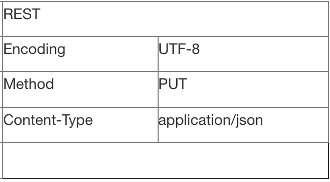
\includegraphics[scale = 1]{assets/diagrams/STPRequestParams.png}
    \caption{. Dispersion Service REST API Headers}\label{fig:STPRequestParams}
\end{figure}

The specific interface required for the request must include all the necessary banking data for a payment order to be processed.[3]\\

Any bad request should be handled accordingly in Atrato’s server, but when the request is done correctly STP can respond with the following interface:

\begin{verbatim}
    {
       result: { id: number; errorDescription?: string }; 
    }
\end{verbatim}
  
The field id can be interpreted differently depending on its length. According to STP’s documentation, any number greater tan 3 digits refers to the internal reference to the newly generated payment order; if the id is lower or equal to 3 digits, then it serves as an error code which should be consulted in STP’s errors catalog. Whenever the data received refers to an error, the field errorDescription will include additional details regarding the specific response, otherwise, it will not be included in the response.\\

This service will be consumed when the balance system's trigger succesfully generates a Bank Transfer and the dispatch is either automatically triggered or manually confirmed. The system will then proceed to generate a payment order and send it through STP. The specific processes required after STP has confirmed thar the payment order was successfully generated are described in Figure \ref{fig:stp_send_payment_order}.

\begin{figure}[H]
    \centering
    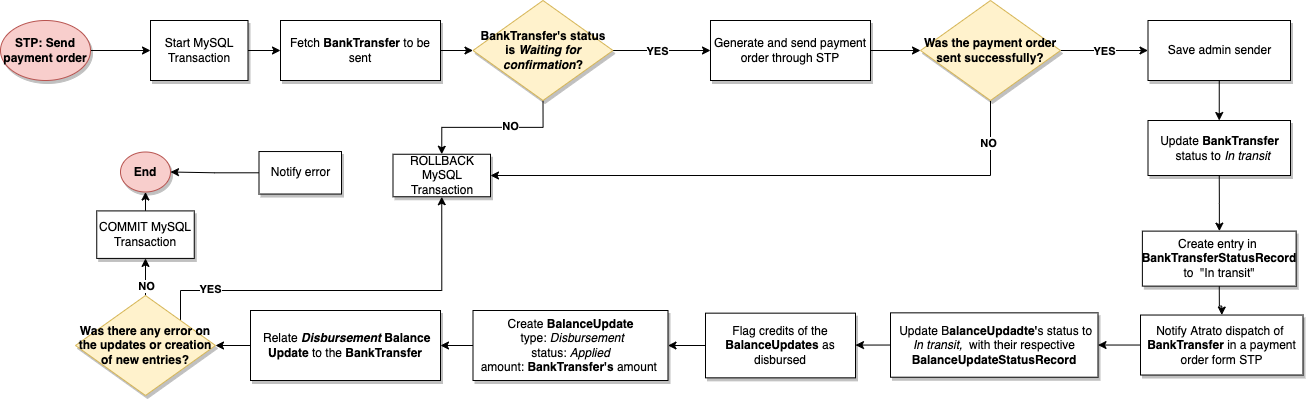
\includegraphics[scale = 0.3]{assets/flowcharts/STP_Send_Payment_Order.png}
    \caption{Balance}\label{fig:stp_send_payment_order}
\end{figure}

\section{Webhooks for Bank Transfers Status Updates}

Atrato will eventually receive an update on the status of every payment order sent through STP, which will serve as reference on how to handle the Balance Updates and Bank Transfers of every store’s balance system.\\

These status updates will be notified through a webhook that will be available through a virtual private network between Atrato’s sever and STP. Depending on the specific status updates that are received is how every balance system will execute specific logic to handle the result of every outgoing Bank Transfer.\\

Exposing this endpoint through the VPN is already a secure method for handling these status updates, nonetheless an additional security secret key generated by Atrato is required for any incoming activity. These keys will be independent for each environment.\\

\subsection{Understanding the different incoming payment order status updates}

There are only 3 different status that can be notified through this webhook: Liquidated, Cancelled or Returned.\\

Each of these different status updates will be handled independently. Whenever a payment order is Liquidated, this means that the money was correctly accepted by the receiving party. If an order is Cancelled, this means that the payment order was not even dispatched, hence, the money never left Atrato’s bank account. For the Returned status, this means that the money did leave the account, but for any external reason it had to be returned.\\

All the processes resultant of any status update will follow the same general structure and implementation as all the balance system. This means, that any error on the process will log everything on the Logs table and since everything is part of a SQL Transaction, no single object involved will be edited nor created due to the Transaction’s Rollback event. Additionally, the internal status of numerous Balance Updates and Bank Transfers will be updated; every time that this updates occur, new entries will be generated in the Balance Updates and Bank Transfers Status Record tables to keep a complete track of how each status changed over time.\\

Every Bank Transfer object generated and stored in Atrato’s database that is already sent through STP as a payment order will have the status In transit, as explained in Chapter 3. Hence, every incoming status update will trigger specific pipelines to a Bank Transfer whose current is In transit. The status to which the Bank Transfer object can changed are furtherly described in this chapter.\\

Every status update will generate an entry in the Logs table with the purpose of keeping a record of every incoming activity form STP. This will be useful for debugging any unexpected or unusual behavior in the balance system of every store.\\

The webhook exposed for these status updates works with a Switch Case architecture, with specific pipelines for every status update. Additionally, a default case as security to monitor any unexpected activity on the web service as shown in the following code snippet:\\

\begin{verbatim}
switch (statusUpdate) {
    case STPResponseStates.CANCELLED:
     await BankTransfersController.cancelSTPBankTransfer(
      bankTransfer.id
     );
     break;
 case STPResponseStates.RETURNED:
    await BankTransfersController.rejectBankTransfer(
     bankTransfer.id,
     req.body.causaDevolucion
    );
    break;
 case STPResponseStates.LIQUIDATED:
    await BankTransfersController.confirmBankTransfer(
     bankTransfer.id,
     req.body.tsLiquidacion
    );
    break;
 default:
    await STPController.notifyNotFoundStatusChange(
     req.body,
     bankTransfe?.id
    );
    break;
}

\end{verbatim}

The status of a Bank Transfer cannot deliberately change from one status to another one. There must be specific events or actions that trigger a specific change form one status to another one. These triggers are described in Figure \ref{fig:state_machine_bank_transfers}. Note how a Bank Transfer with status Waiting for confirmation can only be updated either Cancelled or to the status In transit by sending a new payment order through STP. Both states Cancelled and Rejected can be considered as final states, but the state Applied could still be furtherly updated to Rejected. Once a Bank Transfer is Applied, its state could be considered as a final state, but the rare possibility of the money being returned at some point still exists, even months after the confirmation. For this reason, there is an additional trigger that needs to be considered to update a Bank Transfer’s status from Applied to Rejected; this will be furtherly explained below.

\begin{figure}[H]
    \centering
    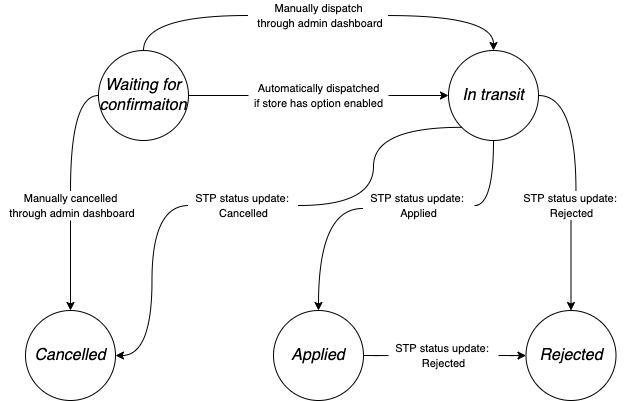
\includegraphics[scale = 0.5]{assets/diagrams/BankTransfersStateMachine.png}
    \caption{Balance Updates State Machine}\label{fig:state_machine_bank_transfers}
\end{figure}

\subsection{Liquidated status update}

This status notifies a successful bank transfer between Atrato and the receiving party. Once this status update is received the Bank Transfer object’s status related to this payment order will now be updated from In transit to Applied and all the Balance Updates that are related to this Bank Transfer will now update their status to Applied as well. Since this means that a disbursement was successfully made, a new Balance Update of type Disbursement, with status Applied, will be created to subtract to the store’s balance the amount of the Bank Transfer. Any Balance Update of type Disbursement that is created must always have their status set to Applied, so that any following Bank Transfer trigger event will not take this Balance Update into account.\\

Furthermore, the credits of which their Balance Update of type Contribution were included in this Bank Transfer can now be flagged as Disbursed. This will only serve as an indication in the merchant’s dashboard showing that these credits have already been disbursed.

\begin{figure} [h]
    \centering
    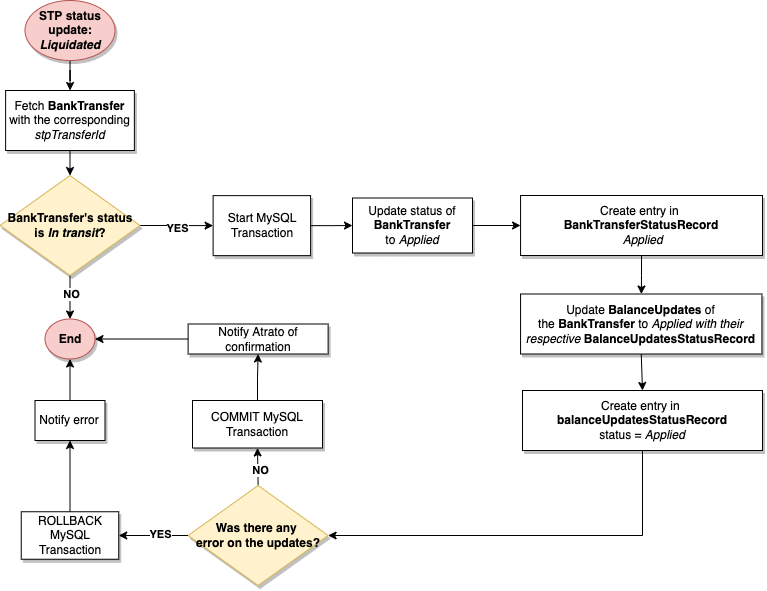
\includegraphics[scale = 0.4]{assets/diagrams/LiquidatedStatusUpdate.png}
    \caption{Processing internal status of Balance Updates and Bank Transfer for Liquidated payment orders}\label{fig:liquidated_status_update}
\end{figure}

\subsection{Cancelled status update}

This status does not happen very often, but still needs to be considered. Whenever a Bank Transfer is cancelled its status will be updated to Cancelled and no further action will be taken regarding a cancelled Bank Transfer, since this is a final state. In terms of the Balance Updates that composed this Bank Transfer, their status will be updated back to Pending, meaning that they could and will be considered for the next Bank Transfer generated once the Bank Transfer’s trigger takes place.\\

This does not necessarily mean that a new Bank Transfer object with the same amount and same related Balance Update objects will be generated because it will depend entirely on the next bank transfer generation event that is triggered and the Balance Updates that have a status of pending by the time the trigger takes place.

\begin{figure} [h]
    \centering
    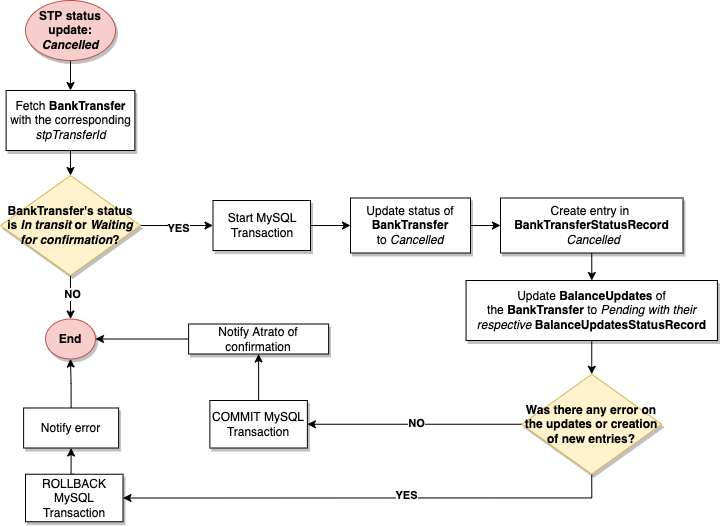
\includegraphics[scale = 0.4]{assets/diagrams/CancelledStatusUpdate.png}
    \caption{Processing internal status of Balance Updates and Bank Transfer for Cancelled payment orders}\label{fig:cancelled_status_update}
\end{figure}

\subsection{Returned status update}

If a payment order is returned, the process that the Bank Transfer object will follow depends on its state. If the state is In transit, meaning it is a Bank Transfer that was recently sent through a payment order, then the Bank Transfer object related to this order will update its status to Rejected and the process regarding to the Balance Updates will be very similar to a cancellation: their status will be updated back to Pending so that they can be considered in a new Bank Transfer in the next trigger. Since no additional updates were made to the store’s general balance then no further action is required, just as in a cancellation.\\

Meanwhile, if the status of the Bank Transfer object is already Applied, then additional to the previous process of updating the Balance Updates back to Pending, further actions need to be taken. Moneywise, the Balance Updates that were previously confirmed, but now the money was returned to Atrato’s account, meaning that they should be considered in a new Bank Transfer.\\

For this specific scenario, a new Balance Update of type Disbursement was already generated when the Bank Transfer was previously confirmed, so a new Balance Update of type Disbursement Override needs to be generated to compensate the changes made to the store’s balance. This new Balance Update will directly update the store’s balance; hence, it will automatically have the status of Applied.\\

By updating the previously confirmed Balance Updates back to Pending, they will eventually be considered into a new Bank Transfer.

\begin{figure} [h]
    \centering
    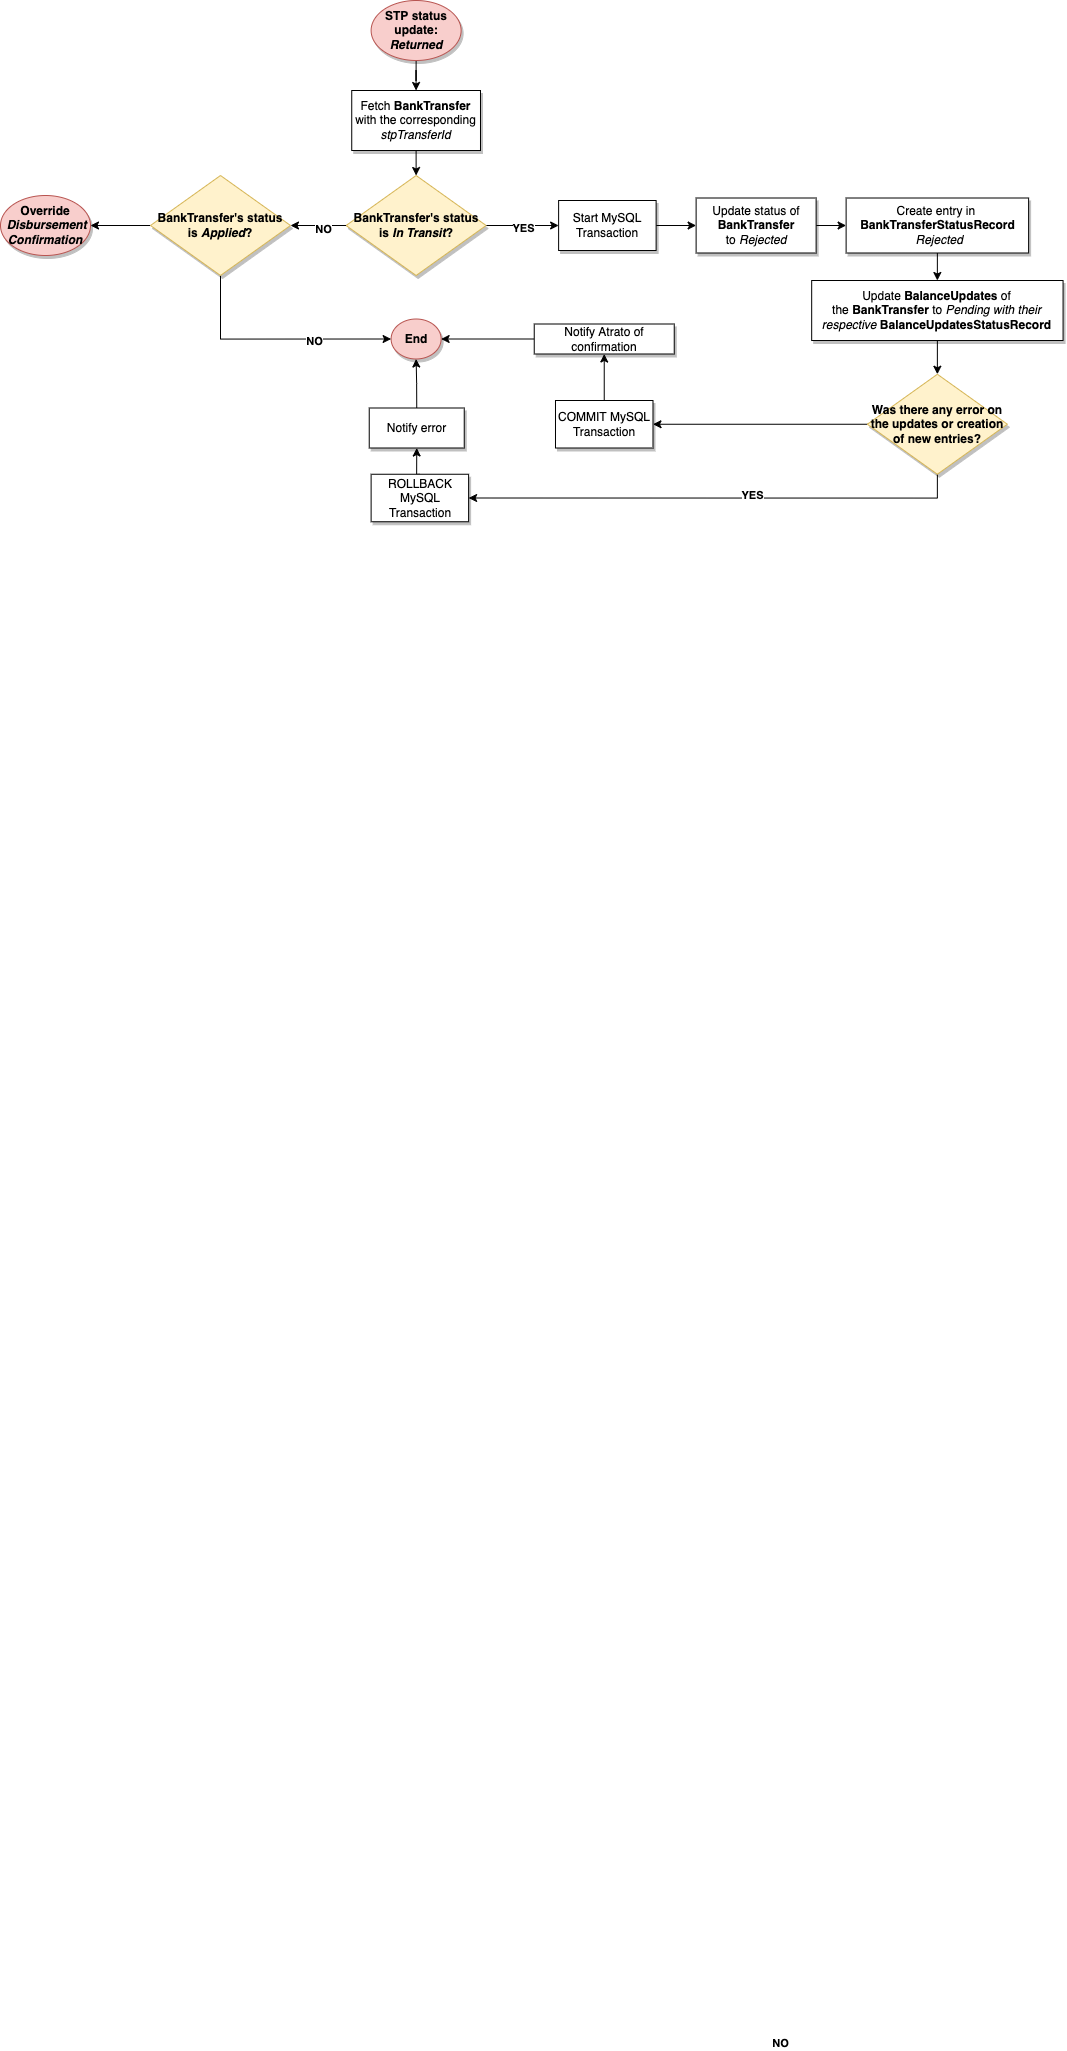
\includegraphics[scale = 0.4]{assets/diagrams/ReturnedStatusUpdate.png}
    \caption{Processing internal status of Balance Updates and Bank Transfer for Returned payment orders. Note the similarity with the Cancelation process}\label{fig:returned_status_update}
\end{figure}


\chapter{Progressive deployment of Balance System}

The transition into a fully automated system, coming from a completely manual process must be done in a progressive way. Every change must be backwards compatible to ensure reliability and to avoid a possible overwhelm due to unknown behaviours. The people involved in this process, in this case the treasury team, must be able to adapt their tasks into this new hybrid system, where some of the tasks are now automated, but others still require their input.

\section{Progressive automation}

In order to progressively migrate into the automation of the credit disbursement process, additional attributes where added into the existing Store entity to be used as variables for either automating or asking for additional validation in some processes: \textit{hasBalanceSystemActive}, \textit{confirmBankTransfersAutomatically}, \textit{mockBankTransferDispatch}. As a good practice, to guarantee the correct handling, identification and manipulation of these variables, a standard naming convention was used, ensuring these attributes where mnemonic, to indicate the observer the intent of its use. \cite{oracle} Key automated actions may or may not require additional validations or confirmation before being executed, such as the dispatch of the bank transfer after it was created, or the mocking of the actual bank transfer. Furthermore, the activation of the balance system for any store also relies on one of these attributes.  This will enable the integration of the automated processes, but still rely on some further manual confirmation or validations if required.\\

\section{Deployment to production}

The process of shipping this new balance system into production consisted in 2 main steps: The deployment of the balance system for some particular stores in an inactive state, and the activation of the system for real bank transfers. Since the balance system is designed to function particularly for every store of Atrato's merchants, simply enabling the system for any store will start to execute the particular actions for each trigger in the system.\\
    
When the system is enabled for a store this means that the every trigger will start to create Balance Updates and generate Bank Transfers accordingly, nonetheless, in order to actually start sending money to from Atrato's bank account to the partners account a second validation must be made. The integration with STP and its Dispersion service can be mocked individually for any store. This means that multiple stores could have the balance system enabled, but none of them will actually send any money unless they have STP active as well. This mock enables the treasury team to start monitoring the real behaviour of the balance system without the risk of making any real bank transaction, just as if the system was in a trial period. In this way, they can ensure mainly that the commisions for any particular store and their active credits are being computed appropiately. Once the correct behaviour and computations of any balance system is confirmed, then the trial period could end by simply activating STP to the system. Now, instead of simply mocking the bank transfer, a real transaction will be made. This two step deployment process will facilitate having control over wich stores' automatic balance system is enabled and also validating wich of these are working appropiately and are ready to be completely automated in production.



\chapter{Discussion and Conclusions}

•Mencionar que tuvimos que entrar un poco al tema de rediseño de las opcoines de pago, pero que se logró independizar, teniendo bien las comisiones todo lo de acá puede funcionar. Los primeros errores que llegamos a notar fue justo eso, que la comision se guardó mal y nos da seguridad de que el sistema si jala chido. Resolviendo el tema de las comisiones, de manera independeinte, el sistem debe de jalar al cien con los cálculos. \\

With the Balance Updates structure, keeping track of how a store's balance changes over time became a simple task. Every new credit contribution, cancelation, disbursement or manual update is directly reflected on the balance. However, managing the grouping of these Balance Updates into Bank Transfer objects was handled with two different approaches:\\

First, the deciding factor on how to group them together was the status of each Balance Update. Whenever the Bank Transfer generation was triggered, either by the CRON JOB execution or by the credit contribution for the immediate dispersion modality, the system computed the amount of the Bank Transfer by taking all the Balance Updates which had a status \textit{Pending} and sum the amount on each of them. These pending Balance Updates could both be the most recently added as well as some that where previously considered for a different Bank Transfer that was either cancelled or rejected and had returned to a the \textit{Pending }status.\\ 

With this approach, the store's real balance was not directly reflected on the last Balance Update, but should be calculated without considering all those Balance Updates with a Status Different than \textit{Applied}. In this scenario, a Bank Transfer could already been generated and sent through STP, but the changes where not reflected on the store's balance until STP confirmed the correct reception of the money. This always left a floating balance that could be later altered depending on the incoming status updates from STP. If for any reason one of the Bank Transfered was cancelled, then all those balance updates returned to the \textit{Pending} status, and could later be considered for another Bank Transfer. The dinamism in the status of the Banlance Updates could add certain level of complexity when computing how the amount for the Bank Transfer was generated.\\ 

In terms of mapping how the Balance Updates where related to the Bank Transfers the status worked perfectly, but to know the real balance of the store, multiple factors needed to be considered. The last Balance Update could indicate an actual balance of \$0.00, but if any previous Balance Update still had the status \textit{In transit}, then the real balance differed.\\ 

This complexity was not noted until a real edge-case, that was not previously considered, happend in production: for any Bank Transfer that was sent through STP a status update was expected. If none was recived, then the Balance Updates that generated that Bank Transfer will always remain with a status \textit{In transit}, and they will always appear as a pending movement for the store. If the bank transfer was cancelled, days after it was sent, then probably more Balance Updates and even Bank Transfers would have already been created by the time of the cancellation. If this was the case, then by the event of the next trigger for the Bank Transfer generation, all those previously generated Balance Updates would merge with the most recent ones to compose a new Bank Transfer, which was exactly the expected behaviour: to include in any new Bank Transfer all those Balance Updates that where still pending with the objetive of leaving none of them pending at all. As stated before, the status were very helpful to relate Balance Updates and Bank Transfers correctly, but the amount for the Bank Transfer could be complicated to decompose.\\

The ambiguity and the complex traceablity in the computation of the amount for every Bank Transfer led to the second approach: to keep the mapping and grouping of Balance Updates and Bank Transfers through their status, but consider always the store's actual balance for any new Bank Transfer. Furthermore, an additional change in the logic was required: unlike the first alternative, a Balance Update of type \textit{Disbursement} is now immediately generated once a Bank Transfer is sent, instead of waiting for STP's confirmation. With this approach, the store's actual balance, taken from the last Balance Update, is always considered for the amount of the next Bank Transfer. Once this newly generated Bank Transfer is sent, the \textit{Disbursement} Balance Update will be immediately generated, bringing the store's balance back to \textit{\$0.00}.\\ 

For stores with their balance system set up for immediate disbursements, unless an external event occurs such as possible cancelations or adjustments, their system will always be showing the following behaviour: an increase in the balance being affected by credit contributions and immediately a disbursement bringing the balance back down.\\


Additionally, if any of the Bank Transfers that were sent is later cancelled, a new Balance Update should be generated to compensate the changes in the store's balance already made by the \textit{Disbursement} Balance Update. This changes enable a much clearer understanding and breakdown of the store's balance in relation with every Bank Transfer that is sent. A cancellation of a Bank Transfer is very easy to understand, unlike with the previous appoach, where a cancellation would only bring back the status of the Balance Updates to \textit{pending}, and later assign them to a new Bank Transfer.\\ 

The change in the approach to this much simpler and undestandable algorithm was mainly triggered by some unexpected behaviour in STP's integration. The edge-case where no status update was received was never considered, and since its some responsibility of a third party then these actions rely outside of our area of control.\\ 

For such integrations and automated processes, it is of utmost importance to be able to track every trigger, action and result inside the processes occuring. By keeping a log of everything that is happening it is easier to monitor that everything is working as expected. Whenever an action is triggered, some very specific results should be happening, and when these results do not proceed as planned, then through these logs its easier to decid wether it is an error in the system that needs to be fixed or it is an error in the action that was triggered. Even for stores that do not have the balance system enabled, keeping  a log of how processes are interrupted is very important and these interruptions do not necessarily indicate an error, but on the contrary, that the system is disabled and will not proceed with the execution of the actions unless it is activated.

\section{Conclusion}

Automation in Atrato's business processes is a key factor for the scalability of current operations and even the final product for customers and partners. Now that the last step of the whole pipeline has been included in the automation, the next steps towards the growth that Atrato's customers and partners have been demanding should not be set back by operational load. To acomplish this, it was necessary to redefine and establish certain guidelines and procedurees for these operations. A process that is not clearly defined can and should not be automated, otherwise the outcomes could be very unpredictable. For this reason the first step, before even attempting to design and define the balance system for stores, was to define the current business process for the disbursements, analyze its limitations and define hould these could be addressed.\\

The whole commission and special promotions handling that was taking place in the commercial area could have been the rabbit hole that would prevent the successful automation of these processes. It was during the computation of the exact amount that needed to be disbursed per credit where most anomalies or differences where happening. By detaching the commission definition from the credit disbursement process, the latter could now be succesfully analyzed, addressed and automated.\\

By attempting to automate this process, as an indirect result, the whole disbursement operation was analyzed and redefined to become much simpler and well established. With the objective not to magnify the process' innefficiency, first it was necessary to define a very efficient pipeline and then proceed to automate and enhance this efficiency.\\

Furthermore, by integrating a third party service for the connection with the mexican digital banking system as part of the autmation of the balance system, possible external errors or misfunctions should also be considered. In other words, the system should be able reliable enough and should not interrupt internal processes when third party integrations are not working as expected. Every possible point of failure of the system was be thoroughly analyzed and the solutions were planned accordingly, such as the case where status updates on STP could not be received.\\

To be able to maintain a high level of traceablity throughout any store's balance system the use of Atrato's internal logging system was very helpful. Designing every controllers internal methods to implement the logger and always keep track of completed and interrupted processes with their corresponding payload for additional details was key for catching errors at early stages of development and even after deployment. Additionally, the use of query runners and MySQL Transactions is very useful for either completing a whole procedure or not at all. This left no uncomplete changes in the database and uncompleted processes or actions could be later addressed and retried.\\

Finally, the proposed solution to this manual and extensive process was successfully designed and developed: an automated system that could handle a store's balance and its changes through different internal and external triggers and actions to periodically or sistematically disburse the corresponding amount for the Atrato's partners' customers' purchases. Until now, one partner with three stores is already implementing this automation with real bank transfers. And a second partner, with more than 40 stores, is in the first process of validating their balance systems. More than 2.4 Million mexican pesos have already been processed through the system through 250+ bank transfers, the amount of which can be broken down into their corresponding individual Balance Updates.\\

These balance systems where integrated with existing business processes to enable a smooth and progressive transition into a fully automated system. By having the option of disabling and enabling these automations at any time, the whole process became completely backwards compatible in case it is necessary.\\


\section{Further Work}

A very interesting next approach to these balance systems would be to review the possibility to manage them not individually by store, but in a more general way by merchants. A merchant could have many stores, but it could be the same banking information and the same people managin all these stores. For these particular cases, it would be very convinient to manage all bank transfers from all these stores as part of one unified balance system. This balance will now be significant to the merchant itself, but keeping track of how every store contributed to the merchant's balance. This could add an additional layer of complexity to the whole system, but if designed appropiately, could also be very easy to handle and manage.\\ 

On the other hand, apart from the Dispersion service, STP provides a variety of services regarding the mexican digital banking system, not only for transfering money between banking accounts but also many interesting digital financial services that could possibly even open the opportunity for new products within Atrato's scope. As part of this integraiton, the connection was already established, making the implementation and integration of new services just a manner of further development that could be done.\\

Coming back to the development of the balance system, as part of the main objectives was to keep traceability of the processes at all times. Many of the design patterns and implementations used for these modules could be extended to further parts of Atrato's internal application. Designing systems where no processes are left incomplete and always accounting for external factors could lead to a very robust, reliable and scalable application. Atrato's next big challenges will not only involve further automations, but also building systems that support the scalability that is needed. Existing on-going business processes are going to need to stay up to date with Atrato's growth and start to be defined considering these factors in order to be able to be scaled without the need to grow the oprational team. A very efficient process with a very efficient team enhanced with the correct tools will be able to extend and keep the same high standard and top performance that is always expected.
% \chapter{Methods}

% This chapter is about methodology and discusses research strategies, data collection methods and data analysis methods. A simple overview of the relationships between these is given in Figure \ref{fig:methods}.


% \section{Research approach/study design}

% Lorem ipsum dolor sit amet, consectetur adipiscing elit, sed do eiusmod tempor incididunt ut labore et dolore magna aliqua. Ut enim ad minim veniam, quis nostrud exercitation ullamco laboris nisi ut aliquip ex ea commodo consequat. Duis aute irure dolor in reprehenderit in voluptate velit esse cillum dolore eu fugiat nulla pariatur. Excepteur sint occaecat cupidatat non proident, sunt in culpa qui officia deserunt mollit anim id est laborum.

% \section{Study setting}

% Lorem ipsum dolor sit amet, consectetur adipiscing elit, sed do eiusmod tempor incididunt ut labore et dolore magna aliqua. Ut enim ad minim veniam, quis nostrud exercitation ullamco laboris nisi ut aliquip ex ea commodo consequat. Duis aute irure dolor in reprehenderit in voluptate velit esse cillum dolore eu fugiat nulla pariatur. Excepteur sint occaecat cupidatat non proident, sunt in culpa qui officia deserunt mollit anim id est laborum.

% \section{Data collection}

% Lorem ipsum dolor sit amet, consectetur adipiscing elit, sed do eiusmod tempor incididunt ut labore et dolore magna aliqua. Ut enim ad minim veniam, quis nostrud exercitation ullamco laboris nisi ut aliquip ex ea commodo consequat. Duis aute irure dolor in reprehenderit in voluptate velit esse cillum dolore eu fugiat nulla pariatur. Excepteur sint occaecat cupidatat non proident, sunt in culpa qui officia deserunt mollit anim id est laborum.

% \section{Data analysis}

% Lorem ipsum dolor sit amet, consectetur adipiscing elit, sed do eiusmod tempor incididunt ut labore et dolore magna aliqua. Ut enim ad minim veniam, quis nostrud exercitation ullamco laboris nisi ut aliquip ex ea commodo consequat. Duis aute irure dolor in reprehenderit in voluptate velit esse cillum dolore eu fugiat nulla pariatur. Excepteur sint occaecat cupidatat non proident, sunt in culpa qui officia deserunt mollit anim id est laborum.

% \section{Ethical considerations}

% Lorem ipsum dolor sit amet, consectetur adipiscing elit, sed do eiusmod tempor incididunt ut labore et dolore magna aliqua. Ut enim ad minim veniam, quis nostrud exercitation ullamco laboris nisi ut aliquip ex ea commodo consequat. Duis aute irure dolor in reprehenderit in voluptate velit esse cillum dolore eu fugiat nulla pariatur. Excepteur sint occaecat cupidatat non proident, sunt in culpa qui officia deserunt mollit anim id est laborum.


% \chapter{Results}


% This chapter can present the results of the study. Tables are often helpful for presenting results. For example, have a look at Table \ref{tab:titles1}.

% Hello


% \section{Subheading}

% Lorem ipsum dolor sit amet, consectetur adipiscing elit, sed do eiusmod tempor incididunt ut labore et dolore magna aliqua. Ut enim ad minim veniam, quis nostrud exercitation ullamco laboris nisi ut aliquip ex ea commodo consequat. Duis aute irure dolor in reprehenderit in voluptate velit esse cillum dolore eu fugiat nulla pariatur. Excepteur sint occaecat cupidatat non proident, sunt in culpa qui officia deserunt mollit anim id est laborum.

% \section{Subheading}

% Lorem ipsum dolor sit amet, consectetur adipiscing elit, sed do eiusmod tempor incididunt ut labore et dolore magna aliqua. Ut enim ad minim veniam, quis nostrud exercitation ullamco laboris nisi ut aliquip ex ea commodo consequat. Duis aute irure dolor in reprehenderit in voluptate velit esse cillum dolore eu fugiat nulla pariatur. Excepteur sint occaecat cupidatat non proident, sunt in culpa qui officia deserunt mollit anim id est laborum.


% \chapter{Discussion}

% This chapter could discuss your work. Comparing the results of your work to those of  previous studies is one important part of the discussion. See how this can be done in 
% \cite{Simon1996-hh} and \cite{Hevner2004-wq}.

% \section{Subheading}

% Lorem ipsum dolor sit amet, consectetur adipiscing elit, sed do eiusmod tempor incididunt ut labore et dolore magna aliqua. Ut enim ad minim veniam, quis nostrud exercitation ullamco laboris nisi ut aliquip ex ea commodo consequat. Duis aute irure dolor in reprehenderit in voluptate velit esse cillum dolore eu fugiat nulla pariatur. Excepteur sint occaecat cupidatat non proident, sunt in culpa qui officia deserunt mollit anim id est laborum.

% \chapter{Conclusion}

% Lorem ipsum dolor sit amet, consectetur adipiscing elit, sed do eiusmod tempor incididunt ut labore et dolore magna aliqua. Ut enim ad minim veniam, quis nostrud exercitation ullamco laboris nisi ut aliquip ex ea commodo consequat. Duis aute irure dolor in reprehenderit in voluptate velit esse cillum dolore eu fugiat nulla pariatur. Excepteur sint occaecat cupidatat non proident, sunt in culpa qui officia deserunt mollit anim id est laborum.

% \textbf{Note about referencing:} \textit{In LaTex, literature references are handled by creating a BibTeX file and referring to it. From Google Scholar, you can grab BibTeX references by clicking on "Import into BibTeX" below a search result. You can also generate BibTeX files from reference managers, such as Mendeley, Paperpile or Zotero.}


% %%%%%%%%%%%%%%%%%%%%%%%%%%%%
% % REFERENCES
% %%%%%%%%%%%%%%%%%%%%%%%%%%%%

% % \addtocontents{toc}{\bigskip}
% \addcontentsline{toc}{part}{Bibliography}


% %%%%%%%%%%%%%%%%%%%%%%%%%%%%
% % APPENDICES
% %%%%%%%%%%%%%%%%%%%%%%%%%%%%

% \appendix
% \cleardoublepage
% % \addtocontents{toc}{\bigskip}
% \addcontentsline{toc}{part}{Appendices}

% %% OPTIONAL - Max 10-15 pages in total

% \chapter{Appendix title}

% \chapter{Another Appendix}


\end{document}